\documentclass[a4paper]{article}

\usepackage[margin=3cm]{geometry}

% the last of the arguments is the default language
\usepackage[ngerman,english]{babel}

% header and footer
\usepackage{fancyhdr}

\usepackage[utf8]{inputenc}

\usepackage[pdftex]{graphicx}

% we need to use 'minipage' for figures (instead of the 'figure' environment).
% hence, we need the 'captionof' command (part of the 'caption' package).
\usepackage{caption}

\usepackage{xcolor}

% code background
\definecolor{code}{gray}{.95}

% create diagrams
\usepackage{tikz}

%\usepackage{hyperref}
\usepackage[pdftex,
            pdfauthor={Secure by Default, Inc.},
            pdftitle={Penetration Test Report},
            pdfsubject={How I Hacked The Worst Company Ever!},
            pdfkeywords={},
            pdfproducer={LaTeX},
            pdfcreator={pdflatex}]{hyperref}
            
% inline code
\newcommand{\passthrough}[1]{\colorbox{code}{\lstset{mathescape=false}#1}}

% define level-4 section
\usepackage{titlesec}
\setcounter{secnumdepth}{4}
\titleformat{\paragraph}
  {\normalfont\normalsize\bfseries}{\theparagraph}{1em}{}
  \titlespacing*{\paragraph}
  {0pt}{3.25ex plus 1ex minus .2ex}{1.5ex plus .2ex}

% Pandoc uses '\tightlist' inside list environments
\def\tightlist{}

% disable indentation of first line of paragraphs
\usepackage{parskip}

% nice code listings
\usepackage{listings}
\lstset{
  backgroundcolor=\color{code},
  basicstyle=\footnotesize\ttfamily,
  upquote=true,
  linewidth=\textwidth,
  breaklines,
  breakatwhitespace,
  frame=single,
  numbers=none,
}

% severity gauge
%
%              7
% ||||||||||||||......
% 0                 10
\newcommand{\severitygauge}[3][1]{
  \begin{tikzpicture}[scale=#1]
    % bounding box
    \path (-3,0) (13,0);

    % empty rectangle
    \filldraw[fill=white, draw=black] (0, -0.1) rectangle (10, 0.1);

    % filled rectangle, showing the gauge's measurement
    \filldraw[fill=black, draw=black] (0, -0.1) rectangle (#2, 0.1);

    % range of the gauge
    \path (0, -0.2) node[anchor=north]{0};
    \path (10, -0.2) node[anchor=north]{10};

    % the gauge's measurement as text
    \path (#2, 0.2) node[anchor=south]{#3};
  \end{tikzpicture}
}

% minimal severity gauge: without range and textual measurement.
% horizontal
\newcommand{\minmalseveritygaugeH}[2][1]{
  \begin{tikzpicture}[scale=#1, baseline=-0.5ex]
    \filldraw[fill=white, draw=black] (0, -0.3) rectangle (10, 0.3);
    \filldraw[fill=black, draw=black] (0, -0.3) rectangle (#2, 0.3);
  \end{tikzpicture}
}

% minimal severity gauge: without range and textual measurement.
% vertical
\newcommand{\minmalseveritygaugeV}[2][1]{
  \begin{tikzpicture}[scale=#1]
    \path (0, 0) (0, 12); % bounding box
    \filldraw[fill=white, draw=black] (-0.5, 0) rectangle (0.5, 10);
    \filldraw[fill=black, draw=black] (-0.5, 0) rectangle (0.5, #2);
  \end{tikzpicture}
}




 % -------------------- GAUGE BAR SSVC --------------------------------
\newcommand{\severitygaugeSSVC}[2][1]{
  \begin{tikzpicture}[scale=#1]
    % bounding box
    \path (-1,0) (5,0);

    % empty rectangle
    \filldraw[fill=white, draw=black] (0, -0.1) rectangle (4, 0.1);

    % filled rectangle, showing the gauge's measurement
    \filldraw[fill=black, draw=black] (0, -0.1) rectangle (#2, 0.1);

    % range of the gauge
    \path (1, -0.2) node[anchor=north]{Track};
    \path (2, -0.2) node[anchor=north] {Track*}
    \path (3, -0.2) node[anchor=north] {Attend}
    \path (4, -0.2) node[anchor=north]{Act};

  \end{tikzpicture}
}






% conditionals (in macros)
\usepackage{etoolbox}

\newcommand{\highlight}[3]{
  \ifstrequal{#2}{#3}{\framebox{#1}}{#1}
}

\newcommand{\CVSStwo}[7]{
  \begin{tabular}{ll}
    \textbf{Access Vector} & \textbf{Confidentiality Impact}
    \\
    \highlight{Local}{L}{#2} \hspace{0.5em} \highlight{Adjacent Network}{A}{#2} \hspace{0.5em} \highlight{Network}{N}{#2}
    \hspace{2em}
    &
    \highlight{None}{N}{#5} \hspace{0.5em} \highlight{Partial}{P}{#5} \hspace{0.5em} \highlight{Complete}{C}{#5}
    \vspace{1.5ex}
    \\
    \textbf{Access Complexity} & \textbf{Integrity Impact}
    \\
    \highlight{High}{H}{#3} \hspace{0.5em} \highlight{Medium}{M}{#3} \hspace{0.5em} \highlight{Low}{L}{#3}
    \hspace{2em}
    &
    \highlight{None}{N}{#6} \hspace{0.5em} \highlight{Partial}{P}{#6} \hspace{0.5em} \highlight{Complete}{C}{#6}
    \vspace{1.5ex}
    \\
    \textbf{Authentication} & \textbf{Availability Impact}
    \\
    \highlight{Multiple}{M}{#4} \hspace{0.5em} \highlight{Single}{S}{#4} \hspace{0.5em} \highlight{None}{N}{#4}
    \hspace{2em}
    &
    \highlight{None}{N}{#7} \hspace{0.5em} \highlight{Partial}{P}{#7} \hspace{0.5em} \highlight{Complete}{C}{#7}
  \end{tabular}
}

\newcommand{\CVSSthree}[9]{
  \begin{tabular}{ll}
    \textbf{Attack Vector} & \textbf{Scope}
    \\
    \highlight{Network}{N}{#2} \hspace{0.5em} \highlight{Adjacent}{A}{#2} \hspace{0.5em} \highlight{Local}{L}{#2} \hspace{0.5em} \highlight{Physical}{P}{#2}
    \hspace{2em}
    &
    \highlight{Unchanged}{U}{#6} \hspace{0.5em} \highlight{Changed}{C}{#6}
    \vspace{1.5ex}
    \\
    \textbf{Attack Complexity} & \textbf{Confidentiality}
    \\
    \highlight{Low}{L}{#3} \hspace{0.5em} \highlight{High}{H}{#3}
    \hspace{2em}
    &
    \highlight{None}{N}{#7} \hspace{0.5em} \highlight{Low}{L}{#7} \hspace{0.5em} \highlight{High}{H}{#7}
    \vspace{1.5ex}
    \\
    \textbf{Privileges Required} & \textbf{Integrity}
    \\
    \highlight{None}{N}{#4} \hspace{0.5em} \highlight{Low}{L}{#4} \hspace{0.5em} \highlight{High}{H}{#4}
    \hspace{2em}
    &
    \highlight{None}{N}{#8} \hspace{0.5em} \highlight{Low}{L}{#8} \hspace{0.5em} \highlight{High}{H}{#8}
    \vspace{1.5ex}
    \\    
    \textbf{User Interaction} & \textbf{Availability}
    \\
    \highlight{None}{N}{#5} \hspace{0.5em} \highlight{Required}{R}{#5}
    \hspace{2em}
    &
    \highlight{None}{N}{#9} \hspace{0.5em} \highlight{Low}{L}{#9} \hspace{0.5em} \highlight{High}{H}{#9}
  \end{tabular}
}

\newcommand{\DREAD}[5]{
  \begin{tabular}{lccc}
    \textbf{Damage}          & \highlight{Low}{L}{#1} & \highlight{Medium}{M}{#1} & \highlight{High}{H}{#1} \\
    \textbf{Reliability}     & \highlight{Low}{L}{#2} & \highlight{Medium}{M}{#2} & \highlight{High}{H}{#2} \\
    \textbf{Exploitability}  & \highlight{Low}{L}{#3} & \highlight{Medium}{M}{#3} & \highlight{High}{H}{#3} \\
    \textbf{Affected Users}  & \highlight{Low}{L}{#4} & \highlight{Medium}{M}{#4} & \highlight{High}{H}{#4} \\
    \textbf{Discoverability} & \highlight{Low}{L}{#5} & \highlight{Medium}{M}{#5} & \highlight{High}{H}{#5} 
  \end{tabular}
}



\newcommand{\SSVCtwo}[7]{
  \begin{tabular}{ll}
    \textbf{Exploitation} & \textbf{Automable}
    \\
    \highlight{PoC}{P}{#1} \hspace{0.5em} \highlight{Active}{A}{#1} \hspace{0.5em} \highlight{None}{N}{#1} \hspace{0.5em} \highlight{Physical}{P}{#2}
    \hspace{2em}
    &
    \highlight{Yes}{Y}{#2} \hspace{0.5em} \highlight{No}{N}{#2}
    \vspace{1.5ex}
    \\
    \textbf{Technical Impact} & \textbf{Mission and Well-Being}
    \\
    \highlight{Partial}{P}{#3} \hspace{0.5em} \highlight{Total}{T}{#3}
    \hspace{2em}
    &
    \highlight{Low}{L}{#6} \hspace{0.5em} \highlight{Medium}{M}{#6} \hspace{0.5em} \highlight{High}{H}{#6}
    \vspace{1.5ex}
    \\
    \textbf{Decision} 
    \\
    \highlight{Track}{T}{#7} \hspace{0.5em} \highlight{Track*}{R}{#7} \hspace{0.5em} \highlight{Attend}{A}{#7} \hspace{0.5em} \highlight{Act}{C}{#7}
  \end{tabular}
}




% align columns at decimal points
\usepackage{dcolumn}
\newcolumntype{d}[1]{D{.}{.}{#1}}

% nicer tables
\setlength{\tabcolsep}{10pt} % increase horizontal spacing; default value: 6pt
\renewcommand{\arraystretch}{1.5} % increase vertical spacing; default value: 1
\begin{document}

% header and footer
\pagestyle{fancy}
\fancyhf{} % clear existing header/footer entries

\begin{titlepage}

  \vspace*{\fill}

  \begin{center}
    \makebox[\textwidth]{
\includegraphics[width=\paperwidth]{templates/title}}
  \end{center}

  \vfill
  
  {
    \Huge \textbf{\MakeUppercase{Penetration Test Report}}
    \vspace{1ex}
  }

  {
    \Large \textbf{Evil Corp, Inc.}
    %\vspace{1ex}
  }

  {
    \Large \textbf{How I Hacked The Worst Company Ever!}
    %\vspace{1ex}
  }

  2024-04-10
\end{titlepage}

\fancyhead[L]{How I Hacked The Worst Company Ever!}
\fancyhead[R]{Confidential}

\fancyfoot[C]{\thepage}

{
  \vspace*{\fill}

  This report is for the sole information and use of Evil Corp, Inc.

  \textbf{Secure By Default, Inc.} \\
  \href{tel:+0123456789}{+0 123 456 789} \\
  \href{mailto:contact@sbd.local}{contact@sbd.local} \\
  \href{https://sbd.local/}{https://sbd.local/}
}

\clearpage
\section*{Executive Summary}
%\addcontentsline{toc}{section}{Executive Summary}

Evil Corp, Inc.\ (i.e.\ the customer) engaged Secure By Default, Inc.\ to conduct a penetration test on their systems.
In accordance with the customer the following types of penetration tests have been conducted:

\begin{itemize}
      \item Add a new vulnerability rating system to the ``report-generator''

      \item 5 Vulnerabilities Report

  \end{itemize}



%+++++++++++++++++++++JUST WITH CVSS++++++++++++++++++++++++++++++++++++++++++++

 Vulnerabilities with severity scores between Track and Act (on a scale from Track--Act) have been found (see Table~\ref{tab:vulnerabilities}).
  A detailed list thereof, including descriptions on how they were found, and recommendations for mitigations, can be found in Section~\ref{sec:results}.


  \begin{table}[h!]
    \centering
    \caption{The vulnerability classes, the highest Decision, and the number of issues per class.}
    \label{tab:vulnerabilities}
    \begin{tabular}{lcr}
      \textbf{Class} & \textbf{Highest Decision} & \textbf{Issues} \\
      \hline
              Class Container & Attend} & 1 \\
              Class Deserialization & Track} & 1 \\
              Class Hijacking & Act} & 1 \\
              Class Injection & Attend} & 1 \\
              Class Phishing & Act} & 1 \\
            \hline
      \textbf{Total} & ~ & \textbf{5}
    \end{tabular}
  \end{table}

%+++++++++++++++++++++JUST WITH SSVC (DONE!)++++++++++++++++++++++++++++++++++++++++++++


My first taks was to implement a new flag on the ``report-generator'' tool. This
flag (-s/--scoretype) should handle different Severity Score from \textbf{CVSS} which is
the standard on this tool. I have made my own researchs about \textbf{CVSS} issues and why
is not always ideal before find a different score type. \textbf{CVSS} is an industry standard
maintained by NVD which define vulnerability as :

\emph{``A weakness in the computational logic (e.g., code)
fouund in software and hardware components that, when exploited, results in a negative impact to confidentiality,
integrity, or availability. Mitigation of the vulnerabilities in this context typically involves coding changes,
but could also include specification changes or even specification deprecations (e.g., removal of affected protocols
or functionality in their entirety).''}

The point of scoring vulnerability is to prioritize patching process, obviously based on the \emph{``danger''} (yes, this
word needs more context to be defined but allow me to use it out of context for the sake of discussion) of each vulnerability.
\textbf{CVSS is not a Risk Score} but a snapshot in time on how the vulnerability is in a specific software/platform/OS/ecc..
This create a small but focal gap to reflect reality of things, when a vulnerability is patched the CVSS score will
decrease even if the patcher entity grade it as higher (see CVE-2023-35352 affecting Microsoft RDP, CVSS score of 6.5
but CRITICAL for Microsoft). Moreover is a quantitative approach used to prioritize the patching checklist (in the case of Microsoft RDP vuln,
using CVSS would delay the fix even the high rate of threat) and cannot be ideal to client with lack of knowledge aout how
CVSS score works, looking just at the numbers and create a leaderboard based solely on them. Lastly the context is not properly involved
in the classification, every network is different and a CVSS of 9/10 in an enviroment could rely with proper detection/prevention technique or
in an unimportant assets (in term of security/CIA triad) making the exploit of the vuln not that dangerous as the score rapresentation.
With ``context'' we mean not just the victim environment but how much the vuln is exploited in the wild or existence of a public PoC,
this should be considered into the evaluation to help clients to improve the security posture.

I have looked through some alternatives and I decide to use one which looks pretty interesting, this doesn't mean is ideal for the industry
use but I wanted to implement something different and new. I decided to use SSVC (CVSS but the opposite way), a decision tree apporach which result
is a categorical variable called \textbf{Decision}. Stakeholder Specific Vulnerability Categorization leverage the vulnerability prioritizing methods
involving stakeholders involved during th patching process, this new side introduction alone make it really different from the simple CVSS number.
The results is based on decision tree which can be used for every gap found into the victim environment and should take care of the big picture not
just the vulnerability itself. This would mark the same vulnerability inside \emph{hMail} different for equal vuln inside \emph{OutLook}, taking into account
how the vulnerable assets is used inside the client \emph{``mission''}. I used the \href{https://www.cisa.gov/ssvc-calculator}{CISA SSVC calculator} because is simple
and concise, the Decision Tree can be summarized like it follows:

\begin{itemize}
\tightlist
\item
  \textbf{State of Exploitation} = present state of the vuln (not future prediction); \emph{None}, \emph{PoC} or \emph{Active}
\item
  \textbf{Automable} = difficult and speed of exploitation and consequent actions; \emph{Yes} or \emph{No}
\item
  \textbf{Techical Impact} = can be compared on CVSS severity score, how much control the Threat get after exploitation; \emph{Partial} or \emph{Total}
\item
  \textbf{Mission \& Well-Being} = the sum of 2 categorical variable (Mission Prevelance + Well-Being Impact); \emph{Low}, \emph{Medium} or \emph{High}
\end{itemize}

The full information can be found \href{https://www.cisa.gov/sites/default/files/publications/cisa-ssvc-guide\%20508c.pdf}{here} on how the decision tree work.
Obviously different trees can be developed (because stakeholder change) so SSVC is not a one-shot solution itself and ad-hoc decision tree could be created
for specific type of clients (private company, public institution, critical infrastructure, ecc..). The peculiarity of such system is the results at the end
of the tree, a category not a number. It would not just prioritize but also suggest how to behave on every vulnerabiliy found, you could make a checklist and
work concurently on every issues with an horizontal approach (with proper attention) for everyone inside the patching process:

\begin{itemize}
\tightlist
\item
  \textbf{Track} = No action but track the vulnerability situation. Consider to change your approach based on the new informations (for instance a public PoC or APT use)
\item
  \textbf{Track+} = Like \emph{Track} but monitor it closely and be prepared for future changes
\item
  \textbf{Attend} = Actively request info about this vulnerability and assistance as well, notify (at least) internals about it giving the right attention. Actions should be done
\item
  \textbf{Act} = Every stakeholder must be notified in order to meet and plan short-term mitigation/prevention technique.
\end{itemize}

The SSVC CISA score is similar to the CVSS with obviously no numbers but \textbf{Decison Value}, in the \emph{issues files} have been saved like the following under the \emph{severity section} :

\begin{lstlisting}
Track
SSVCv2/E:P/A:Y/T:T/P:M/B:M/M:L/D:T
\end{lstlisting}

Regarding the challenge itself, working with categorical data forced me to make important addition (no copy-\&-paste with parameter changes) on the whole repository (all python and latex files have been touched).
I have explored the whole workflow of the script and learn some python usage new for me (Jinja2 was not that easy to understand at the start), I tried to change just the essential
part of the repository to maintaint the identity of the codes and recognize immediately the changes and how they melt with pre-exisisting task. Same thing applied for the template and style
of final PDF.

(Note that I have manually changed some SSVC string manually to have it all of the same length, this is because different path in the tree may return more value insidethe SVVC string
so consider this as a beta. I worked under an assumption that a standardize tree have been implemented so all SSVC string have same length making copy-paste enough)


\clearpage
\tableofcontents

\clearpage
\section{Introduction}

Evil Corp, Inc.\ (i.e.\ the customer) engaged Secure By Default, Inc.\ to conduct a penetration test on their systems.
In accordance with the customer the following types of penetration tests have been conducted:

\begin{itemize}
      \item Add a new vulnerability rating system to the ``report-generator''

      \item 5 Vulnerabilities Report

  \end{itemize}

\subsection{Personnel}

The following people were involved in this penetration test:

\begin{itemize}
      \item Alessio Stefan (alessiosteph@proton.me)

  \end{itemize}

\subsection{Scope}

Between yyyy-mm-dd and yyyy-mm-dd the following components have been analyzed:

\begin{itemize}
      \item \passthrough{\lstinline!evil-corp.com!} (application server)

      \item \passthrough{\lstinline!https://4ever-evil.com/!} (web application + API)

  \end{itemize}

All test-related IP traffic originates from the following addresses:

\begin{itemize}
  \item \passthrough{192.168.0.0/24}
\end{itemize}

\subsection{Methodology}

As asked by Patrick Himler I would grab 5 vulnerabilities found in my (little) CTF experience. This
vulnerabilities would be managed as stand-alone so obviously the report sections are not connected to
each others and are part of different machine. I would use the template to make a brief description of every vulnerability context so you can make an idea of the rating I gave to them, since I am not that keen with SSVC you could expect unaccurate results. I will explain briefly why I choose a specific path in the Decision tree to make it clear also I will try to use all the capabilities provided by the tools (image, link, snippet of code).

  \subsection{Requirements}

  Secure By Default required the following from the customer:

  \begin{itemize}
          \item technical contact personnel: fulfilled

          \item user accounts (at least two per type) for the web application: fulfilled

          \item API access token: fulfilled

          \item \href{https://www.openapis.org/}{OpenAPI Specification} document for the API: none provided

      \end{itemize}

  \subsection{Provided Information}

  The customer has provided the following additional information:

  \begin{itemize}
          \item source code of the web application

          \item Apache config

      \end{itemize}

  \subsection{Limitations}

  Due to the time-constrained nature of audits, it is common to encounter coverage limitations.
  The following limitations were identified during this engagement.
  Secure By Default recommends further review and/or retesting of the affected systems/components.

  \textbf{Dapibus}

In dapibus est nec elit fermentum, et lacinia ipsum auctor.
Praesent rhoncus, metus a tempor ultricies, ex ligula consequat elit, non sollicitudin massa libero vel odio.
Duis blandit cursus metus.
Quisque ac tincidunt lorem.
Cras laoreet urna sed mi sagittis, et sagittis enim mattis.
Praesent porttitor, dolor sagittis egestas hendrerit, ex neque sagittis sapien, vel tincidunt dui libero et sem.
Fusce a odio faucibus, finibus augue non, aliquam augue.

\textbf{Convallis}

Nulla vitae nunc at magna molestie sodales convallis non libero.
Pellentesque nec lectus lacinia, ultricies nulla in, laoreet lectus.
Mauris eget urna efficitur, hendrerit diam eu, gravida mi.
Phasellus porta lacinia ligula, ut dictum mi viverra at.
Nullam dictum eros vitae massa ultrices, ac iaculis ante rhoncus.
Donec pellentesque nec est sed porta.


\subsection{Tools}

The following tools have been used during the engagement:

\begin{itemize}
\tightlist
\item
  Nmap: network scanner
\item
  cURL: command-line tool for transferring data using various network protocols
\item
  Impacket-Suite: Set of tools for Active Directory enumeration/exploitation
\item
  Burp Suite: web application security scanner
\item
  ysoserial: Malicious serialization string crafter
\item
  ffuf: Web Fuzzer written in Go
\item
  Chisel: Port Forwarding tool taht support both TCP and UDP over HTTP
\item
  Hydra: Cuncurrent bruteforcing tool supporting various protocols
\item
  Metasploit: The most famous exploit framework you can find online! (it really needs presentation? lol)
\item
  Responder: LLMNR/NBT-NS/mDNS Poisoner that support HTTP,SMB, webDAV and others protocol to use as rogue
\item
  Hashcat: The most dangerous cat in the Kali Linux tools repository (ミ⚈ﻌ⚈ミ)
\item
  \LaTeX: document preparation
\end{itemize}


\clearpage

\section{Results}
\label{sec:results}



        %+++++++++++++++++++++++++++ JUST CVSS ++++++++++++++++++++++
        %+++++++++++++++++++++++++++ JUST CVSS ++++++++++++++++++++++








        %+++++++++++++++++++++++++++ JUST SSVC ++++++++++++++++++++++


        \begin{table}[h!]
        \centering
        \caption{Vulnerabilities and their severity (component ``ANALYSIS'').}
        \begin{tabular}{ p{0.65\linewidth} c d{1} }

          

          \textbf{Vulnerability} & \textbf{Decision} \\
          \hline
                      \hyperref[1:ANALYSIS:issue.md]{[ANALYSIS] LDAP Injection} & Attend \\


                  \end{tabular}
      \end{table}
          \begin{table}[h!]
        \centering
        \caption{Vulnerabilities and their severity (component ``POV'').}
        \begin{tabular}{ p{0.65\linewidth} c d{1} }

          

          \textbf{Vulnerability} & \textbf{Decision} \\
          \hline
                      \hyperref[2:POV:issue.md]{[POV] Insecure Deserialization} & Track \\


                  \end{tabular}
      \end{table}
          \begin{table}[h!]
        \centering
        \caption{Vulnerabilities and their severity (component ``PANDORA'').}
        \begin{tabular}{ p{0.65\linewidth} c d{1} }

          

          \textbf{Vulnerability} & \textbf{Decision} \\
          \hline
                      \hyperref[3:PANDORA:issue.md]{[PANDORA] Path Hijacking} & Act \\


                  \end{tabular}
      \end{table}
          \begin{table}[h!]
        \centering
        \caption{Vulnerabilities and their severity (component ``RUNNER'').}
        \begin{tabular}{ p{0.65\linewidth} c d{1} }

          

          \textbf{Vulnerability} & \textbf{Decision} \\
          \hline
                      \hyperref[4:RUNNER:issue.md]{[RUNNER] Container Administration Commands} & Attend \\


                  \end{tabular}
      \end{table}
          \begin{table}[h!]
        \centering
        \caption{Vulnerabilities and their severity (component ``PREMONITION'').}
        \begin{tabular}{ p{0.65\linewidth} c d{1} }

          

          \textbf{Vulnerability} & \textbf{Decision} \\
          \hline
                      \hyperref[5:PREMONITION:issue.md]{[PREMONITION] Phishing} & Act \\


                  \end{tabular}
      \end{table}
    

        %+++++++++++++++++++++++++++ JUST SSVC ++++++++++++++++++++++


\clearpage


  % loop over each of the group's issues ---------- SERIOUSLY I DON'T UNDERSTAND THIS WTF
      \newpage
    
    \subsection{[ANALYSIS] LDAP Injection}
    \label{1:ANALYSIS:issue.md}

    Similar to SQL or OS injection, LDAP injection use the protocol syntax into a text form (or similar) to
retrieve data stored, commonly, in Active Directory enviroment. This could be really usefull for attackers
who don't have valid credentials to enumerate usernames, password, descriptions and other LDAP field. In
Active Directory we can read every data inside LDAP by design if we have credentials but with this vulnerability
in play threat can circumnavigate this requirement. It become more dangerous with public facing services where
non-authenticated actors could interact freely.

\textbf{Context}

The context is inside the first part of \textbf{Analysis} box, thanks to a nmap scan I was able to identify the presence
of the AD domain called \emph{analysis.htb} and the public machine was the Domain Controller (\emph{dc-analysis.htb}) with a public webapp on port 80.
With some basic enumeration/fuzzing I found the endpoint \textbf{/users} and, more in depth, \textbf{/users/list.php}. Both located into the subdomain \textbf{internal.analysis.htb}
My intuition drove me to add some parameters until the \textbf{?name=} worked properly, with the ``*'' character I got a table with a username
as output. Here I was 100\% sure that LDAP injection attack vector was present (pretty obvious because the same fields in the table are the ones within the AD user catalog) \{\ref{1:ANALYSIS:issue.md:issue11.png}\}.
After exploitation I was able to login in the website backend leveraging my unautenticated situation and move on until foothold thanks to unsafe File Upload
that permits PHP reverse shell to be loaded server-side.


    \subsubsection{Evidence}

          \paragraph{internal.analysis.htb/users/list.php?name=*}

      The user I get on this website endpoint was \textbf{technician}, using \textbf{ASREP-roasting} (\emph{impacket-GetNPUsers} tool) I was able to check if was
a valid user inside the AD domain or not, luckly this was the case \{\ref{1:ANALYSIS:issue.md:issue12.png}\}. At first I tought was SQL because the ``\emph{'' works the same with both LDAP and SQL
but it requir a few tries to understand was LDAP for sure. I had to go AFK and review back LDAP syntax, it required 5/10 minutes and the attack flow
looks clear enough to move on. The server side will just add a parenthesis and doesn't sanitize in any way, changing the parameter with \passthrough{\lstinline!*)(description=*!}
returned the same output, we can enumerate the description of the user \textbf{technician} with adding characters before the last ''}''. I tried manually the first
character to be sure the attack could work and after reciving the output with \passthrough{\lstinline!*)(description=9*!} I know the description start with the character ``9''.
The next step is obvious, we need to automate this process in order tofind the full string (is not uncommon to see plaintext passwords inside the ``description'' field
because the lack of knowledge about who can see what in Active Directory). This is the python script :

\begin{lstlisting}
import string
import request

finish = false
keys = string.ascii_letters + "#$%&'()+,-./:;<->?@[\\]^_{|}*"
url = 'http://internal.analysis.htb/users/list.php?name='
payload = ''
result = ''

while not finish:
    for i in keys:
        print(f'\r{result}{i}', end="")
        payload = result + i
        attack = url + f"*)(description={payload}*"
        resp = requests.get(attack)
        if "technician" in resp.text:
            result = result + i
            break
    finish = False


print(result)
\end{lstlisting}

The results after firing the script is ``97NTtl*4QP96Bv'', this password is not valid for Active Directory Domain but works for the
backend login form (located at \textbf{/employees/login.php}). Here we can upload (and then review) file indiscriminately \{\ref{1:ANALYSIS:issue.md:issue13.png}\}, like a PHP reverse shell that
allowed me to get foothold on the Domain Controller \{\ref{1:ANALYSIS:issue.md:issue14.png}\}.

EXTRA : Before login inside the backend I performed password spraying with the usernames found inside and the password retrieved from the script. The user ``cwilliams'' used the same
pasword which allowed RPC access (but somehow not WinRM). \{\ref{1:ANALYSIS:issue.md:issue15.png}\}

\textbf{SSVC Decision}

\begin{itemize}
\tightlist
\item
  \textbf{Exploitation = PoC}, because \emph{``private evidence of exploitation is tested but not shared''} is true thanks to the costum python script and is a well know attack
\item
  \textbf{Automable = Yes}, the steps 1 to 4 of the kill-chain are fully automable
\item
  \textbf{Technical Impact = Partial}, we retrieved just a specific field of the LDAP records about a single user. Exploiting this doesn't automatically gives you full controll of the vulnerable component
\item
  \textbf{Mission \& Well-Being = High}, the component is directly connected with the client mission (remember this machine is a domain controller)
\item
  \textbf{Decision = Attend}, the sum of the previous choices
\end{itemize}

    
    \subsubsection{Affected Assets}

    \begin{itemize}
\tightlist
\item
  internal.analysis.htb (port 80)
\end{itemize}


    \subsubsection{Severity}

    \begin{center}
      
      %----ADJUST THIS FOR SSVC BUT CHOOSE THE METHOD FOR THE TABLE (WORKE BUT DOUBLE CHECK)----
              \severitygaugeSSVC[2]{3} \newline

        \SSVCtwo{P}{Y}{P}{E}{M}{H}{A}

        


    \end{center}
      % ---------------------------------------------------------------------------------



          \subsubsection{Recommendations}

      \begin{itemize}
\tightlist
\item
  Using LDAP in this tasks is uneccesary risk (especially for a webapp), find alternatives to avoid to make the webapp directly linked with LDAP data also take care of similar solutions inside your environment
\item
  Regardless the origin of data implement sanitization of peculiar character (``)'' for instance) to avoid crafted payload to be injected
\item
  Since the upload form needs to send a file directly to the SoC (and PHP file should be allowed) there is no need to stored in the webserver. Moreover favor private channel rather than backend form to sen this type of files
\item
  Don't use the description field for hardcoded password and avoid password reuse inside your company. The whole password policy needs to be re-designed
\end{itemize}

    
          \subsubsection{References}

      \begin{itemize}
\tightlist
\item
  \href{https://github.com/alstephh/This_Is_Just_A_Hobby/tree/e42a866bb781fb896d6b9c03a33185e192a317b8/MACHINES/HTB/Analysis}{My full walkthrough of Analysis machine}
\end{itemize}

    
          \subsubsection{Images}
      
              \begin{minipage}[c]{\textwidth}
          \centering
          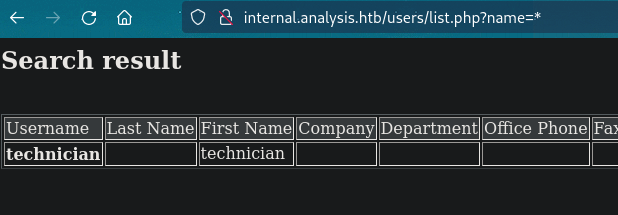
\includegraphics[width=\textwidth]{src/issues/1 - ANALYSIS/issue11.png}
          \captionof{figure}{Output using the "*" as parameter of "name" variable}
          \label{1:ANALYSIS:issue.md:issue11.png}
          \vspace{4ex}
        \end{minipage}
              \begin{minipage}[c]{\textwidth}
          \centering
          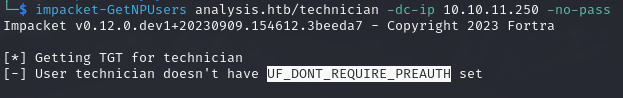
\includegraphics[width=\textwidth]{src/issues/1 - ANALYSIS/issue12.png}
          \captionof{figure}{Check if user "technician" is a valid account inside the AD domain}
          \label{1:ANALYSIS:issue.md:issue12.png}
          \vspace{4ex}
        \end{minipage}
              \begin{minipage}[c]{\textwidth}
          \centering
          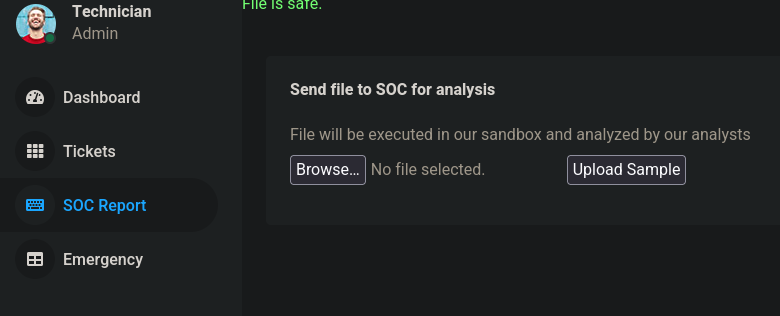
\includegraphics[width=\textwidth]{src/issues/1 - ANALYSIS/issue13.png}
          \captionof{figure}{Upload form within the backend}
          \label{1:ANALYSIS:issue.md:issue13.png}
          \vspace{4ex}
        \end{minipage}
              \begin{minipage}[c]{\textwidth}
          \centering
          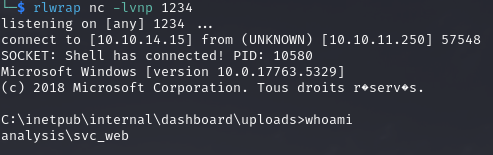
\includegraphics[width=\textwidth]{src/issues/1 - ANALYSIS/issue14.png}
          \captionof{figure}{Reverse shell inside the domain controller}
          \label{1:ANALYSIS:issue.md:issue14.png}
          \vspace{4ex}
        \end{minipage}
              \begin{minipage}[c]{\textwidth}
          \centering
          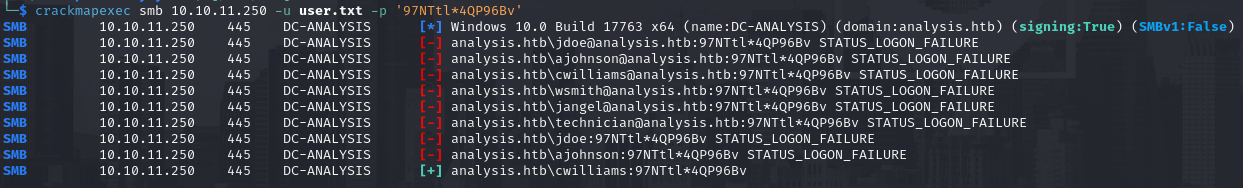
\includegraphics[width=\textwidth]{src/issues/1 - ANALYSIS/issue15.png}
          \captionof{figure}{Password Spraying}
          \label{1:ANALYSIS:issue.md:issue15.png}
          \vspace{4ex}
        \end{minipage}
          
    \clearpage

    

  % loop over each of the group's issues ---------- SERIOUSLY I DON'T UNDERSTAND THIS WTF
      \newpage
    
    \subsection{[POV] Insecure Deserialization}
    \label{2:POV:issue.md}

    Deserialization process take as input a format structured data and rebuilding into an object (eg:/ JSON, XML).
This process is potential harmful when the deserialization string is user-controllable, manipulate the structured data
could lead to command or object injection making the desrialization process the attack vector. Attackers needs to know the
type of deserialization (eg:/ PHP, Java) and craft the serialized object exploiting known gadget that would be handled and
executed by the victim machine (similar to ROP chain). The common impact of this vulnerability is RCE.

\textbf{Context}

Here I will cover the first part of the machine called POV, in order to exploit an ASPX insecure deserialization
you need to find the decryption and validation keys through a LFI. With this 2 requirements I was able to craft
the malicious ASP.NET serialized object that would be injected into the ViewState POST parameter to get a meterpeter
shell.


    \subsubsection{Evidence}

          \paragraph{dev.pov.htb}

      During reconnaissance it has been found that the machine \passthrough{\lstinline!pov.htb!} have only the HTTP service (port 80) open and available to the public. The base
domain is a static brochoure of the website where no interaction can be achieved. Subdomain bruteforcing (with \textbf{ffuf} tool) found \passthrough{\lstinline!dev.pov.htb!} which
look interesting compared to the base domain. Here we have an overview of the (potential) backend technology thanks of a CV which can be downloaded through
the endpoint \passthrough{\lstinline!/portfolio!} \{\ref{2:POV:issue.md:issue21.png}\}. Looking closer the request with BURP the CV file is fetched through a POST parameter (\passthrough{\lstinline!file!}),
I played with this changing the value and discover an LFI and RFI was possible. Knowing this I fired up Responder and use the LFI to fetch a file on the rogue
SMB server in order to grab username and NTLMv2 Hash \{\ref{2:POV:issue.md:issue22.png}\} \{\ref{2:POV:issue.md:issue23.png}\}.
The hash was uncrackable but at least we have harvested a valid machine username, plus inspecting the request highlight the presence of \textbf{ViewState} POST parameter.
\textbf{ViewState} is used for session authenticaion (similar to cookies) and is well known that is vulnerable to \textbf{Insecure Deserialization} when is user controllable but
we need more info about the validation/decryption key/alghorithm if we want to properly inject it without throwing an error. Without covering all the trial-\&-error I made
using the LFI pointing to \passthrough{\lstinline!../web.config!} uncover all the data we need to go further \{\ref{2:POV:issue.md:issue24.png}\}. I create the ASPX malicious object using ysoserial
with the following flags :

\begin{itemize}
\tightlist
\item
  \textbf{-p = ViewState}
\item
  \textbf{-g TextFormattingRunProperties}
\item
  \textbf{--decryptionalg=``AES''}
\item
  \textbf{--decryptionkey=\{AES\_KEY\}}
\item
  \textbf{--validationalg=``SHA1''}
\item
  \textbf{--validationkey=\{SHA1\_KEY\}}
\item
  \textbf{--path=/portfolio/contact.aspx} (can be whatever ASPX page)
\item
  \textbf{-c \{payload for web\_delivery metasploit module\}}
\end{itemize}

Finally we have crafted our own ViewState object and is ready to be injected \{\ref{2:POV:issue.md:issue25.png}\}, now we can make a new request and change the original ViewState
with the crafted one, after that a meterpeter shell as \textbf{web\_svc} user will popout \{\ref{2:POV:issue.md:issue26.png}\}. Foothold has been achieved!

\textbf{SSVC Decision}

\begin{itemize}
\tightlist
\item
  \textbf{Exploitation = PoC}, because \emph{``the vulnerability has a well known method of exploitation''}
\item
  \textbf{Automable = Yes}, we automatically achieved RCE with the successful exploitation of the vulnerability
\item
  \textbf{Technical Impact = Partial}, we are spawning as low privileges user so our potential damage is reduced and need additional steps to go further
\item
  \textbf{Mission \& Well-Being = Medium}, the vulnerable component is a simple workstation with no esential component for the client mission
\item
  \textbf{Decision = Track}, the sum of the previous choices
\end{itemize}

    
    \subsubsection{Affected Assets}

    \begin{itemize}
\tightlist
\item
  dev.pov.htb (port 80)
\end{itemize}


    \subsubsection{Severity}

    \begin{center}
      
      %----ADJUST THIS FOR SSVC BUT CHOOSE THE METHOD FOR THE TABLE (WORKE BUT DOUBLE CHECK)----
              \severitygaugeSSVC[2]{1} \newline

        \SSVCtwo{P}{Y}{P}{S}{M}{M}{T}

        


    \end{center}
      % ---------------------------------------------------------------------------------



          \subsubsection{Recommendations}

      \begin{itemize}
\tightlist
\item
  The LFI is the key factor that allowed insecure deserialization to occur. Instead of using a parameter to fetch the file, create ad-hoc function to grab just the CV without the need of user-controllable parameters
\item
  Never ever deserialize untrusted data, it would not be that simple as it sound but is a risk with relevant consequence
\item
  Check the library used for serialization/deserialization process in order to find some flags/options to prevent code execution
\item
  Removing/Disabling specific gadget can create a cascade effect on the whole infrastructure generating issues and errors. Do it but at your own risk and make proper testing, future implementation could suffer from that so is not suggested if not strictly needed
\end{itemize}

    
          \subsubsection{References}

      \begin{itemize}
\tightlist
\item
  \href{https://github.com/alstephh/This_Is_Just_A_Hobby/tree/main/MACHINES/HTB/POV}{My full walkthrough of POV machine}
\end{itemize}

    
          \subsubsection{Images}
      
              \begin{minipage}[c]{\textwidth}
          \centering
          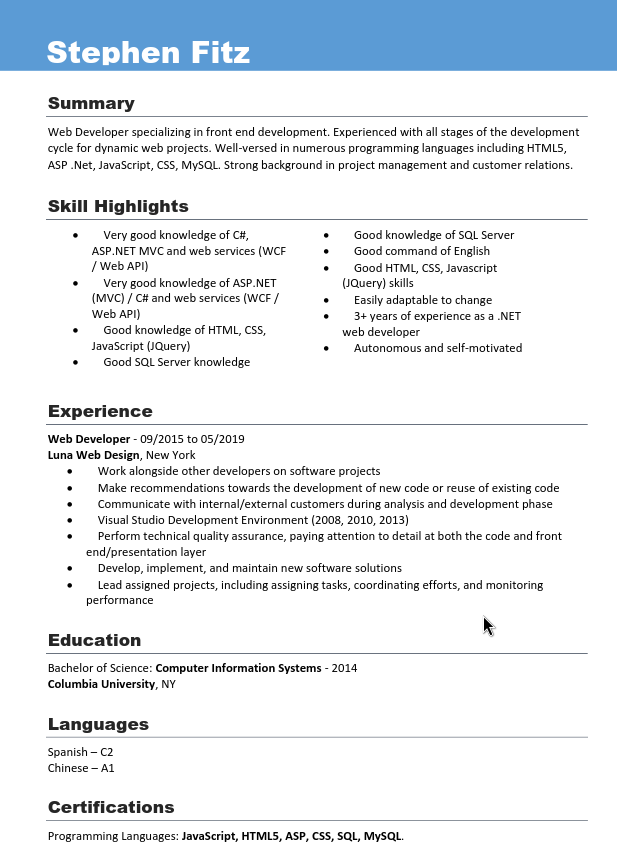
\includegraphics[width=\textwidth]{src/issues/2 - POV/issue21.png}
          \captionof{figure}{CV found into dev.pov.htb}
          \label{2:POV:issue.md:issue21.png}
          \vspace{4ex}
        \end{minipage}
              \begin{minipage}[c]{\textwidth}
          \centering
          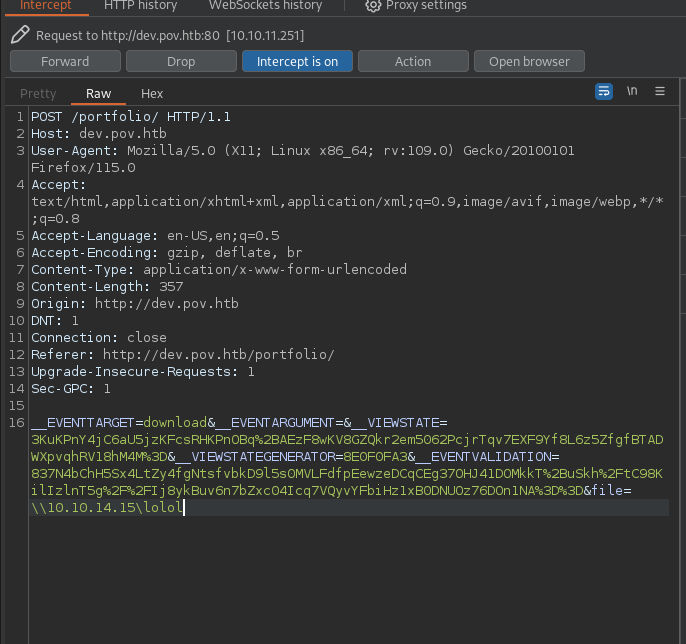
\includegraphics[width=\textwidth]{src/issues/2 - POV/issue22.png}
          \captionof{figure}{LFI/RFI using Burp Suite}
          \label{2:POV:issue.md:issue22.png}
          \vspace{4ex}
        \end{minipage}
              \begin{minipage}[c]{\textwidth}
          \centering
          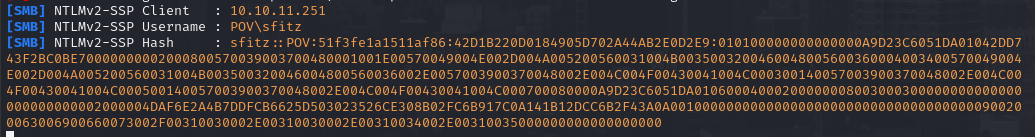
\includegraphics[width=\textwidth]{src/issues/2 - POV/issue23.png}
          \captionof{figure}{NTLMv2 Hash grabbing with Responder}
          \label{2:POV:issue.md:issue23.png}
          \vspace{4ex}
        \end{minipage}
              \begin{minipage}[c]{\textwidth}
          \centering
          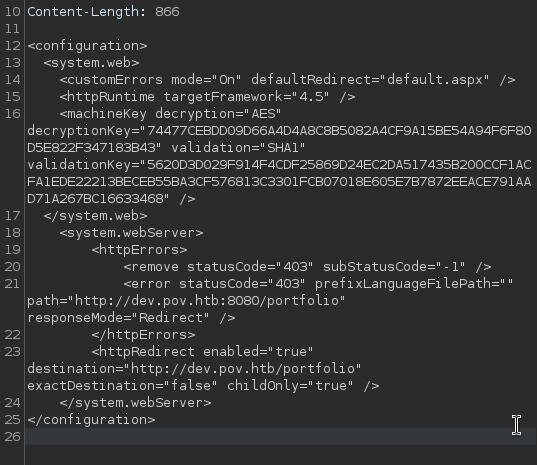
\includegraphics[width=\textwidth]{src/issues/2 - POV/issue24.png}
          \captionof{figure}{Content of the web.conig file discovered through the LFI}
          \label{2:POV:issue.md:issue24.png}
          \vspace{4ex}
        \end{minipage}
              \begin{minipage}[c]{\textwidth}
          \centering
          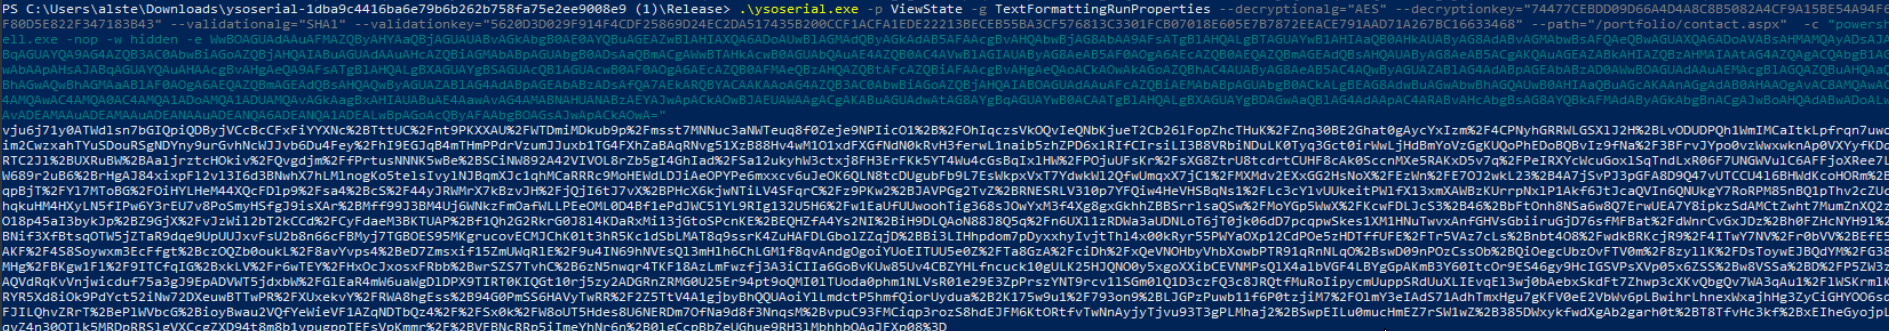
\includegraphics[width=\textwidth]{src/issues/2 - POV/issue25.png}
          \captionof{figure}{Crafting of malicious ViewState string}
          \label{2:POV:issue.md:issue25.png}
          \vspace{4ex}
        \end{minipage}
              \begin{minipage}[c]{\textwidth}
          \centering
          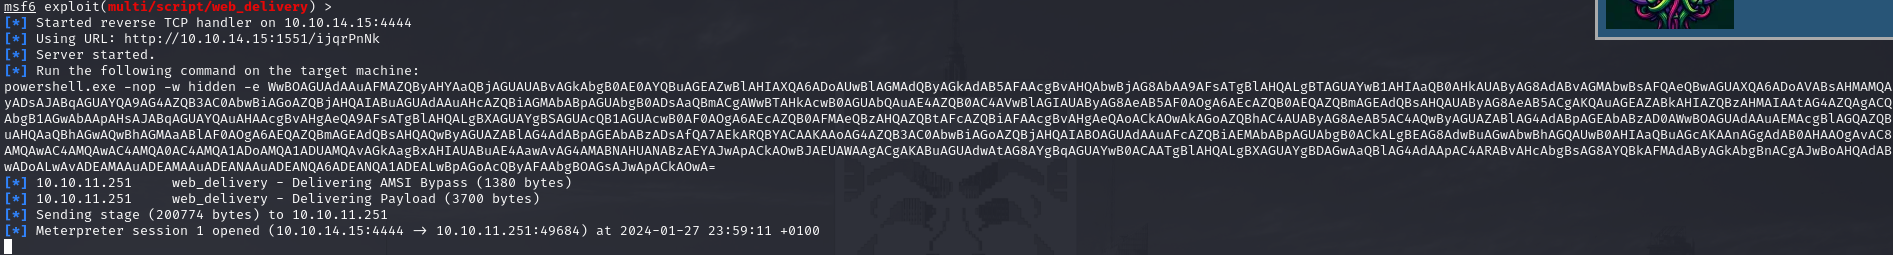
\includegraphics[width=\textwidth]{src/issues/2 - POV/issue26.png}
          \captionof{figure}{Meterpeter reverse shell}
          \label{2:POV:issue.md:issue26.png}
          \vspace{4ex}
        \end{minipage}
          
    \clearpage

    

  % loop over each of the group's issues ---------- SERIOUSLY I DON'T UNDERSTAND THIS WTF
      \newpage
    
    \subsection{[PANDORA] Path Hijacking}
    \label{3:PANDORA:issue.md}

    The use of relative path inside codes could lead to Path Hijacking, the attacker change the \$PATH variable in order
to execute malicious costumversion of program instead the originals one. This doesn't target a specific programming language the
only requirement is to call binaries or program at OS level. The attack is defined under the ``Hijack Execution Flow'' definition where
an attacker abuse a pre-exisisting code in order to perform unwanted action. Is one of the basic methods of Privilege Escalation especially
in Unix system where costum program with SUID/SUDO permissions allow to get root from low privilege users.

\textbf{Context}

Here we will cover the privilege escalation section of th machine \textbf{Pandora}, I get foothold through a well-known exploit of a vulnerable
version of PandoraFMS (\passthrough{\lstinline!v7.0NG.742!}) which is a SQL injection that can be leverage to RCE on the machine. I got access as \passthrough{\lstinline!matt!} user
and found a SUID program which is vulnerable to Path Hijacking to get RCE as \passthrough{\lstinline!root!}.


    \subsubsection{Evidence}

          \paragraph{pandora}

      With simple enumeration it didn't take much before I discovered a costum SUID binary called \textbf{``pandora\_backup''} which is a simple backup
tool for PandoraFMS \{\ref{3:PANDORA:issue.md:issue31.png}\}. Without downloading locally the file and do reverse engineering I tried to use
\passthrough{\lstinline!strings!} linux utility to put an eye of the binary content, luckly it was not that complex and I see the gap that permits exploitation through
Path Hijacking. The binary call \passthrough{\lstinline!tar!} but without the absolute path and without forcing a standard PATH variable inside the code \{\ref{3:PANDORA:issue.md:issue32.png}\}.
I moved into \passthrough{\lstinline!/dev/shm!} and create a version of \passthrough{\lstinline!tar!} that just spawn a bash process, change the PATH enviroment variable giving precedence to this directory
with \passthrough{\lstinline!EXPORT PATH=/dev/shm:$PATH!} and than reuse \passthrough{\lstinline!pandora\_backup!}. This time it will not finish because when it hit \passthrough{\lstinline!tar!} command will spawn a shell as root thanks
to the SUID \{\ref{3:PANDORA:issue.md:issue33.png}\}.

\textbf{SSVC Decision}

\begin{itemize}
\tightlist
\item
  \textbf{Exploitation = Active}, Hijacking Execution flow has been one of the most used technique is \href{https://web.mitre-engenuity.org/hubfs/Center\%20for\%20Threat\%20Informed\%20Defense/CTID-Sightings-Ecosystem-Report.pdf}{2019-2021} even if is reduced is use is one of the favorite tricks by threat in the wild
\item
  \textbf{Automable = No}, the steps from 1 to 4 are not fully automable and requires manual enumeration to discover the vulnerability (like reverse engineering)
\item
  \textbf{Technical Impact = Total}, not just RCE has been achieved but high-level RCE because the SUID that permits to impersonate root user
\item
  \textbf{Mission \& Well-Being = High}, the vulnerable component is not a simple webserver but host the Pandora FMS monitoring software which can lead to remote control of other machines inside the network
\item
  \textbf{Decision = Act}, the sum of the previous choices
\end{itemize}

    
    \subsubsection{Affected Assets}

    \begin{itemize}
\tightlist
\item
  pandora machine
\end{itemize}


    \subsubsection{Severity}

    \begin{center}
      
      %----ADJUST THIS FOR SSVC BUT CHOOSE THE METHOD FOR THE TABLE (WORKE BUT DOUBLE CHECK)----
              \severitygaugeSSVC[2]{4} \newline

        \SSVCtwo{A}{N}{T}{E}{A}{H}{C}

        


    \end{center}
      % ---------------------------------------------------------------------------------



          \subsubsection{Recommendations}

      \begin{itemize}
\tightlist
\item
  Be aware when assign SUID or SUDO permissions to softwares, in this case a backup could be done by a service account or an high-privilege profile which is not root.
\item
  Costum binaries/tool should be full reviewed trying to avoid relative path and add an hardcoded PATH enviroment variable value to guard from Path Hijacking technique, same thing for DLL in Windows
\item
  In general implement the least-privilege principle in every aspects of your infrastructure, if is not a developer account it don't need to cahnge PATH enviroment variable
\end{itemize}

    
          \subsubsection{References}

      \begin{itemize}
\tightlist
\item
  \href{https://github.com/alstephh/This_Is_Just_A_Hobby/tree/main/MACHINES/HTB/Pandora}{My full walkthrough of Pandora machine}
\end{itemize}

    
          \subsubsection{Images}
      
              \begin{minipage}[c]{\textwidth}
          \centering
          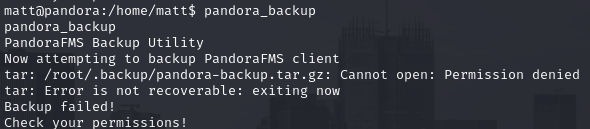
\includegraphics[width=\textwidth]{src/issues/3 - PANDORA/issue31.png}
          \captionof{figure}{A low-priv run of pandora_backup binary}
          \label{3:PANDORA:issue.md:issue31.png}
          \vspace{4ex}
        \end{minipage}
              \begin{minipage}[c]{\textwidth}
          \centering
          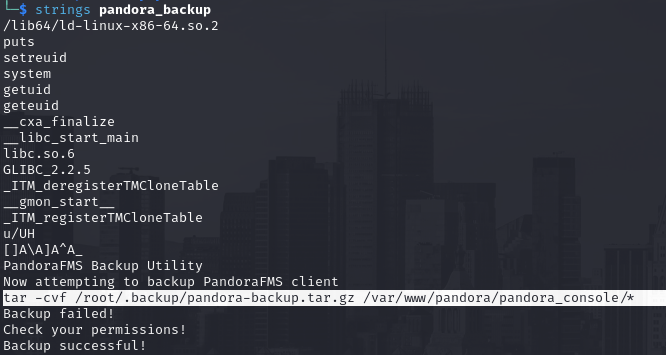
\includegraphics[width=\textwidth]{src/issues/3 - PANDORA/issue32.png}
          \captionof{figure}{Strings of pandora_backup file}
          \label{3:PANDORA:issue.md:issue32.png}
          \vspace{4ex}
        \end{minipage}
              \begin{minipage}[c]{\textwidth}
          \centering
          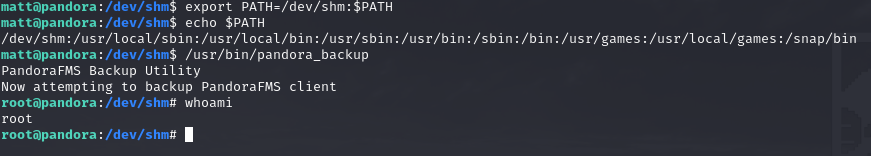
\includegraphics[width=\textwidth]{src/issues/3 - PANDORA/issue33.png}
          \captionof{figure}{Exploitation through Path Hijacking}
          \label{3:PANDORA:issue.md:issue33.png}
          \vspace{4ex}
        \end{minipage}
          
    \clearpage

    

  % loop over each of the group's issues ---------- SERIOUSLY I DON'T UNDERSTAND THIS WTF
      \newpage
    
    \subsection{[RUNNER] Container Administration Commands}
    \label{4:RUNNER:issue.md}

    When adversary put their hands into container administration/orchestration can turn in dangerous consequence. There are various
technique for both RCE and privilege escalation (and more) involving Kubernetes or Docker and companies should be aware of it. From entrypoint
script to container escape makes this technologies a double-edge blade that needs to be handled carefully. Not to mention the flexibility and portability
of containers could be exploited for horizontal movement or pivoting.

\textbf{Context}

\textbf{Runner} machine is a medium machine where the user flag should be grabbed through the exploit of CVE-2024-27918 affecting some TeamCity versions that allows to remotely create
admin users without credentials. After login inside TC a private RSA key has been found and used to SSH inside the machine as \passthrough{\lstinline!john!}. Here Apache configuration file uncover a subdomain
called \passthrough{\lstinline!portainer-administration.runner.htb!} hosting \textbf{portainer.io} docker orchestration software. From here we can deploy pre-existing image into the machine and abusing mount-binding
I was able to retrieve the contents of \passthrough{\lstinline!/root!} folder and grab the flag.


    \subsubsection{Evidence}

          \paragraph{portainer-administration.runner.htb}

      After enumerating the machine internally I visited the \textbf{portainer.io} subdomain which is shielded by the login form \{\ref{4:RUNNER:issue.md:issue41.png}\}. With Hydra I was able to retrieve the
passowrd of one of the users inside the machine, the valid credentials are \passthrough{\lstinline!matthew:piper123!}. Portainer.io is an UI orchestrator for Docker, the trick here is to translate every UI actions to
\passthrough{\lstinline!docker-compose!} flag but looking at the documentation was not that hard. There is justs one predefined image that we can use (a simple \passthrough{\lstinline!ubuntu:latest!}), my first idea was to create a container instance
where can reach a path reachable by the normal user, set a SUID bash as root (in the container) and than execute it in the bare-metal machine. I had some issue with this option (which is still possible) and
decide to abuse \textbf{mount-binding} option to link the \passthrough{\lstinline!/root!} directory to another directory inside the container which, as root, contents can be fetched freely. First I need to create a \href{https://docs.portainer.io/user/docker/volumes/add\#adding-a-tmpfs-volume}{\textbf{tmpfs storage}}
and set it as bind mount \{\ref{4:RUNNER:issue.md:issue42.png}\}. Save the storage and go in the deployment phase, set the storage volume just created and map it to a directory inside the container of your choice \{\ref{4:RUNNER:issue.md:issue43.png}\} and deploy the container
into the machine. When ready, we can finally read the content of the \passthrough{\lstinline!/root!} directory and read the final flag! \{\ref{4:RUNNER:issue.md:issue44.png}\}.

\textbf{SSVC Decision}

\begin{itemize}
\tightlist
\item
  \textbf{Exploitation = PoC}, Portainer.io is really helpfull for the attacker and can modularize the same exploit on different machine
\item
  \textbf{Automable = No}, you need credentials for both the local machine and portainer.io (also not all accounts can perform all the actions), moreover port forwarding is required and the port can change in different networks making hard the creation of a single automation code for this vulnerability
\item
  \textbf{Technical Impact = Total}, in this specific case we can set malicious containers in every machine into the network (in this case the network is a single machine) permitting to move horizontally, vertically and pivoting into other network
\item
  \textbf{Mission \& Well-Being = High}, container are used for different tasks inside the client network and a sabotage of 1+ container can buff threat capabilities
\item
  \textbf{Decision = Act}, the sum of the previous choices
\end{itemize}

    
    \subsubsection{Affected Assets}

    \begin{itemize}
\tightlist
\item
  portainer-administration.runner.htb
\end{itemize}


    \subsubsection{Severity}

    \begin{center}
      
      %----ADJUST THIS FOR SSVC BUT CHOOSE THE METHOD FOR THE TABLE (WORKE BUT DOUBLE CHECK)----
              \severitygaugeSSVC[2]{3} \newline

        \SSVCtwo{P}{N}{T}{E}{A}{H}{A}

        


    \end{center}
      % ---------------------------------------------------------------------------------



          \subsubsection{Recommendations}

      \begin{itemize}
\tightlist
\item
  Check the password policy and implement bruteforcing/logon attempt count mitigation technique even within internal services, a simple solution that can make the attackers life harder
\item
  Monitor properly creation/changes/deployment of new container inside your network and prepare incident response process in case of exploitation attempt
\item
  Container relationships with other network components are complex and a small change could destroy your line of defense, never rely on a single security boundary when protecting from such threat. Meet all the stakeholders involved with containers (users,clients,developers,ecc..) to reach multiple solutions reaching the needs of everyone
\end{itemize}

    
          \subsubsection{References}

      \begin{itemize}
\tightlist
\item
  \href{https://github.com/alstephh/This_Is_Just_A_Hobby/tree/main/MACHINES/HTB/Runner}{My full walkthrough of Runner machine}
\end{itemize}

    
          \subsubsection{Images}
      
              \begin{minipage}[c]{\textwidth}
          \centering
          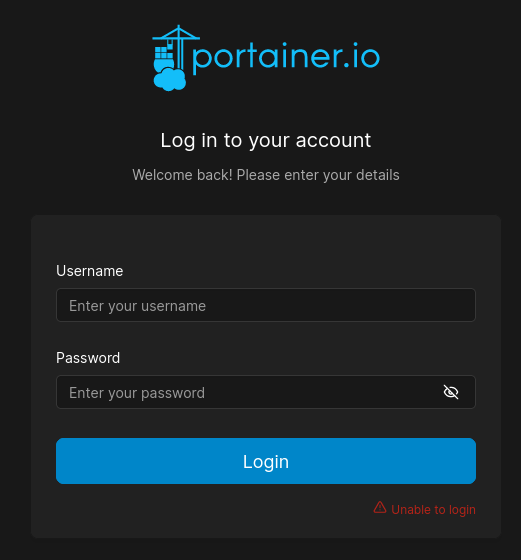
\includegraphics[width=\textwidth]{src/issues/4 - RUNNER/issue41.png}
          \captionof{figure}{Portainer.io subdomain}
          \label{4:RUNNER:issue.md:issue41.png}
          \vspace{4ex}
        \end{minipage}
              \begin{minipage}[c]{\textwidth}
          \centering
          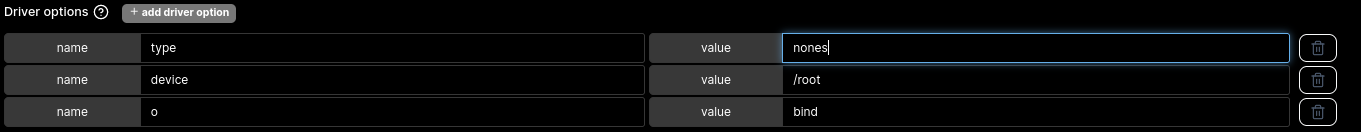
\includegraphics[width=\textwidth]{src/issues/4 - RUNNER/issue42.png}
          \captionof{figure}{Portainer.io Bind Mount creation}
          \label{4:RUNNER:issue.md:issue42.png}
          \vspace{4ex}
        \end{minipage}
              \begin{minipage}[c]{\textwidth}
          \centering
          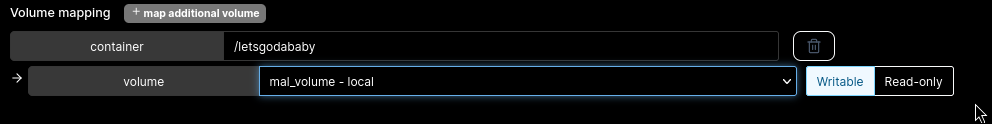
\includegraphics[width=\textwidth]{src/issues/4 - RUNNER/issue43.png}
          \captionof{figure}{Portainer.io storage link with /root flag}
          \label{4:RUNNER:issue.md:issue43.png}
          \vspace{4ex}
        \end{minipage}
              \begin{minipage}[c]{\textwidth}
          \centering
          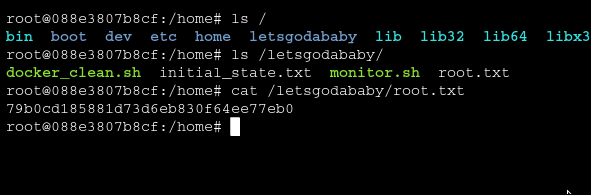
\includegraphics[width=\textwidth]{src/issues/4 - RUNNER/issue44.png}
          \captionof{figure}{Root flag of RUNNER machine read through the container just created}
          \label{4:RUNNER:issue.md:issue44.png}
          \vspace{4ex}
        \end{minipage}
          
    \clearpage

    

  % loop over each of the group's issues ---------- SERIOUSLY I DON'T UNDERSTAND THIS WTF
      \newpage
    
    \subsection{[PREMONITION] Phishing}
    \label{5:PREMONITION:issue.md}

    Phishing needs no presentation is an attack vector known even by non-technical people and is still one of the favorite TTPs by APT. There are different
way to perform it : VBA script, HTA, and XXL are just a few examples that are used for the attack-chain. The general attack flow is the same, we try to convince
the user to download/view/use a malicious attachment delivered in specific way, camouflate as legittimate and automate the malicious actions everything executed with
the right spice of social engineering. Obviously is not simple at it seems other invisible threat (like AV) needs to be handled as well but in this final mini-report I wanted
to cover the first part of the \textbf{Zephyr ProLab} (HackTheBox) where a simple but effective phishing method has been used to get initial access inside the victim network

\textbf{Context}

\textbf{Zephyr} first flag (\emph{The Premonition}) start with just a linux webserver that rely on a full AD infrastructure, through this webserver we can upload PDF for the ``Vacancies'' section, using a crafted
PDF I was able to retrieve NTLMv2 hashes changing the \textbf{/AA} field and pointing it to Responder SMB. The real difference with ``traditional phishing'' (where a sort of reverse shell would occur or fake login form setup)
is that we steal silently without direct user action, just opening the PDF is necessary.


    \subsubsection{Evidence}

          \paragraph{painters.htb}

      Enumeration of \textbf{painters.htb} website (the hostname of the machine is \emph{mail.painters.htb} so my creativity would assume is also a mailserver for the sake of the challenge) ended with the discovery of three different Job Apply form \{\ref{5:PREMONITION:issue.md:issue51.png}\} each of them allow to upload a PDF and send it for review \{\ref{5:PREMONITION:issue.md:issue52.png}\}.
A PDF file can be really threatening when but only with the right information and weaponization. Hacking is not just about tools and techniques (remember what we said about users in the introduction?) but use of simple logic can clean up our head and under-
standing. The ``staff'' would unlikely being some IT guy but maybe someone from HR or non-informatic specialist and we expect this type of professionals to log into SSH on a web
server and use the bash to retrieve our PDF? Probably this PDF would be uploaded on the Linux machine and than passed somewhere else, we in an AD lab so 99\% of chance that
this ``else'' is going to be a Windows machine. With some research I discover the \href{https://www.infosecmatter.com/metasploit-module-library/?mm=auxiliary/fileformat/badpdf}{BADPDF} module in metasploit which would
create (or change) a PDF tuning the \textbf{/AA} field. this field contains 3 different variable:

\begin{itemize}
\tightlist
\item
  \textbf{/S} = The type of action to perform, we would use the GoToR (\emph{Go To Remote}) which would tell the PDF editor the following variable needs to be fetched outside the document (outside means everything, even the machine itself)
\item
  \textbf{/F} = This is the key point, here we can specify a remote file which in our case should be our malicious SMB server \emph{\textbackslash\textbackslash{[}IP{]}\textbackslash{[}FILE{]}}
\item
  \textbf{/D} = The location of the fetched document to extract, not relevant for out purposes
\end{itemize}

The PDF creation is made really simple thanks to metasploit and after generating it we should go and upload on every upload form available to grab as much hash as possible.
After some minutes Responder will start to flood \{\ref{5:PREMONITION:issue.md:issue53.png}\}, that's great! Our intuition was right, the PDF has been opened on a Windows machine!
using \textbf{hashcat} I cracked the Riley hash and get the plaintext (\emph{P@ssw0rd}) and used on the SSH port of the mail/web server, luckly the password policy was not strong enough and allowed to reuse password in this linux machine
and grab the first flag! \{\ref{5:PREMONITION:issue.md:issue54.png}\}.
Later on I have set up this machine as pivot to connect on the internal network and start playing with AD protocols moving further and further.

\textbf{SSVC Decision}

\begin{itemize}
\tightlist
\item
  \textbf{Exploitation = Active}, Phishing is still one of the most used technique in the wild, even with job boards or online forms (look what happened to \href{https://beyondmachines.net/event_details/europol-confirms-portal-hack-claims-no-operational-data-impacted-g-0-8-y-a}{Europol} in these days, lol)
\item
  \textbf{Automable = Yes}, Weaponization, delivery and exploitation are fully automable
\item
  \textbf{Technical Impact = Partial}, retrieving user hash is cool but doesn't automatically means that we have full control on the vulnerable component (the webserver)
\item
  \textbf{Mission \& Well-Being = High}, in this specific case we get controll of the web and mail server with a single stone. These 2 components are foundamental for the security and mission posture of the client
\item
  \textbf{Decision = Act}, the sum of the previous choices
\end{itemize}

    
    \subsubsection{Affected Assets}

    \begin{itemize}
\tightlist
\item
  mail.painters.htb
\end{itemize}


    \subsubsection{Severity}

    \begin{center}
      
      %----ADJUST THIS FOR SSVC BUT CHOOSE THE METHOD FOR THE TABLE (WORKE BUT DOUBLE CHECK)----
              \severitygaugeSSVC[2]{4} \newline

        \SSVCtwo{A}{Y}{P}{S}{I}{H}{C}

        


    \end{center}
      % ---------------------------------------------------------------------------------



          \subsubsection{Recommendations}

      \begin{itemize}
\tightlist
\item
  Is the third time in this paper, password policy needs to be reviewed from the start. No need to use the same passwords into 2 different machine especially if one of them is an important component of the infrastructure
\item
  Zero-Trust approach on everything that originate from the outside, use detection room or sandbox when you need to open unknown files.
\item
  Take care of outgoing and upcoming connection from untrusted source, if there is no needs that a machine inside AD needs to access a public facing SMB use the firewall to kill this connections (same thing applied to similar connections)
\end{itemize}

    
          \subsubsection{References}

      \begin{itemize}
\tightlist
\item
  The ProLab is under paywall and public walkthrough cannot be pubblished until the lab is active. I have attached on the email my full walkthrough in orderto be reviewed without breaking HTB labs
\end{itemize}

    
          \subsubsection{Images}
      
              \begin{minipage}[c]{\textwidth}
          \centering
          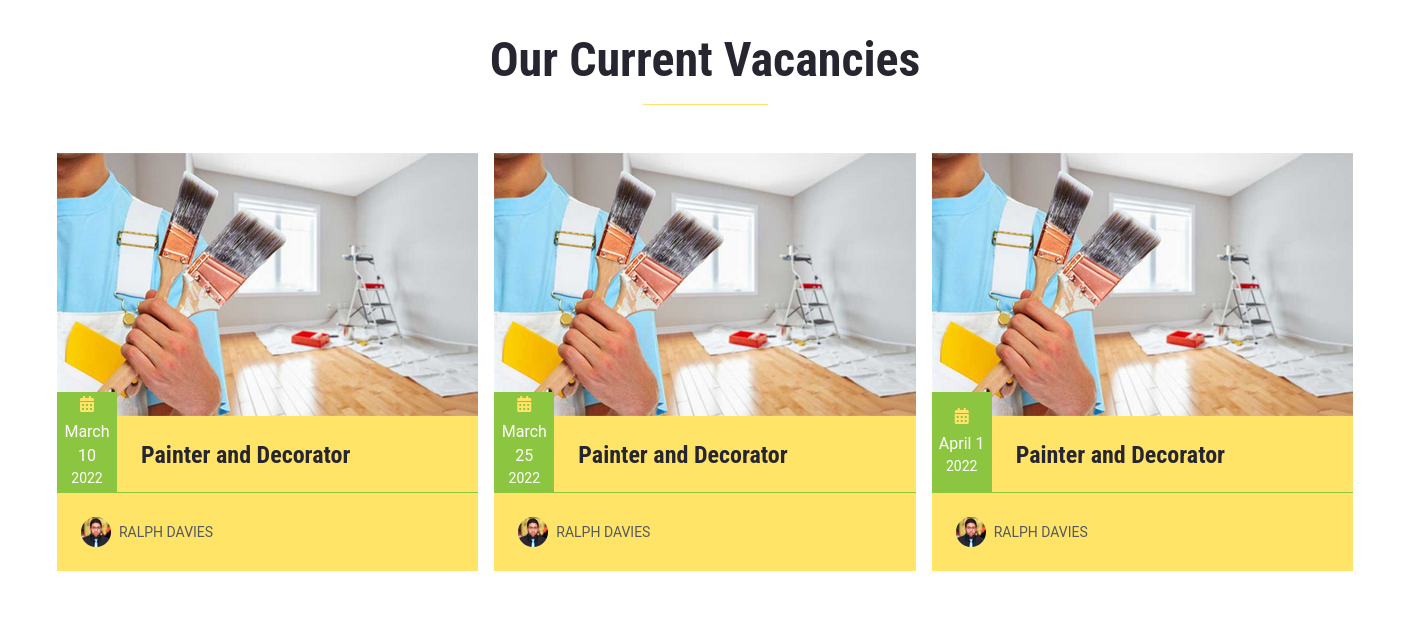
\includegraphics[width=\textwidth]{src/issues/5 - PREMONITION/issue51.png}
          \captionof{figure}{The 3 vacancies sections inside the website}
          \label{5:PREMONITION:issue.md:issue51.png}
          \vspace{4ex}
        \end{minipage}
              \begin{minipage}[c]{\textwidth}
          \centering
          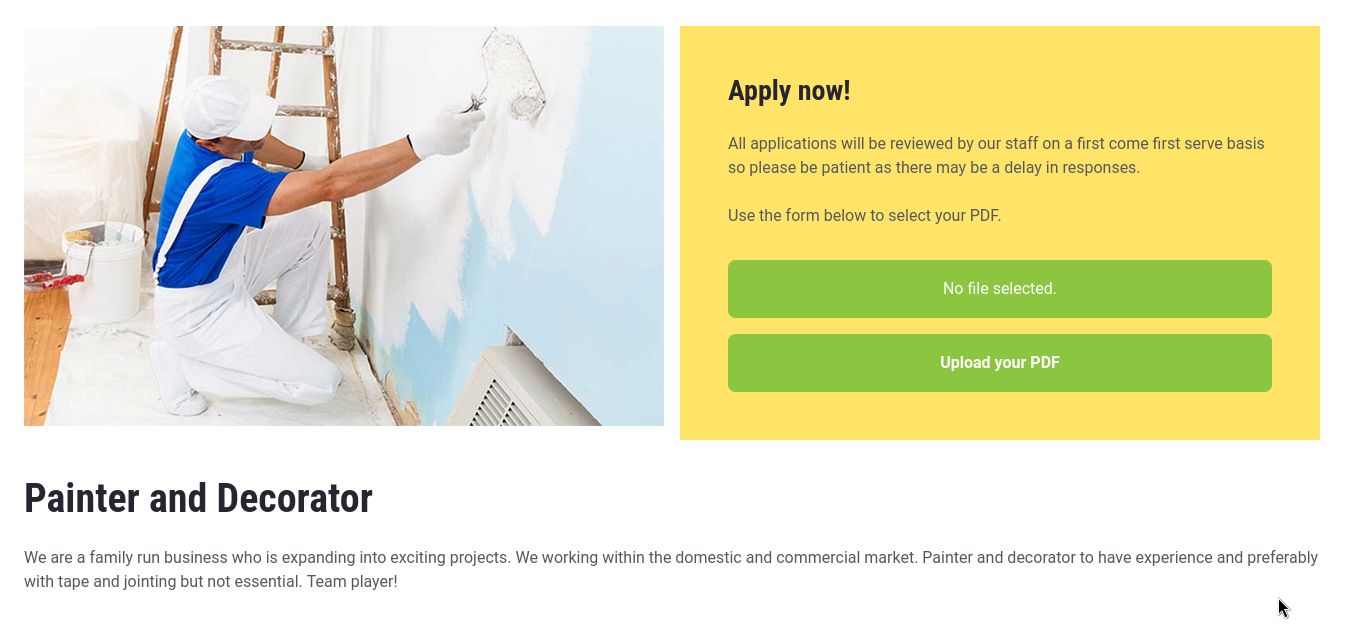
\includegraphics[width=\textwidth]{src/issues/5 - PREMONITION/issue52.png}
          \captionof{figure}{PDF upload form}
          \label{5:PREMONITION:issue.md:issue52.png}
          \vspace{4ex}
        \end{minipage}
              \begin{minipage}[c]{\textwidth}
          \centering
          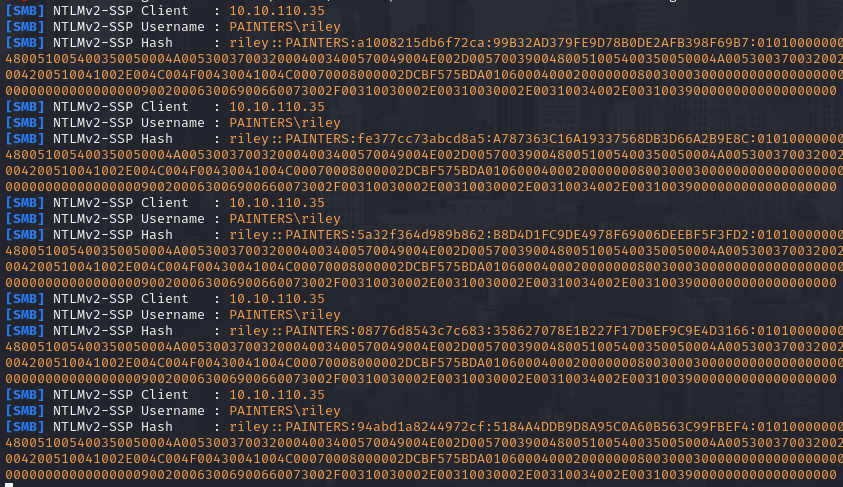
\includegraphics[width=\textwidth]{src/issues/5 - PREMONITION/issue53.png}
          \captionof{figure}{Responder output}
          \label{5:PREMONITION:issue.md:issue53.png}
          \vspace{4ex}
        \end{minipage}
              \begin{minipage}[c]{\textwidth}
          \centering
          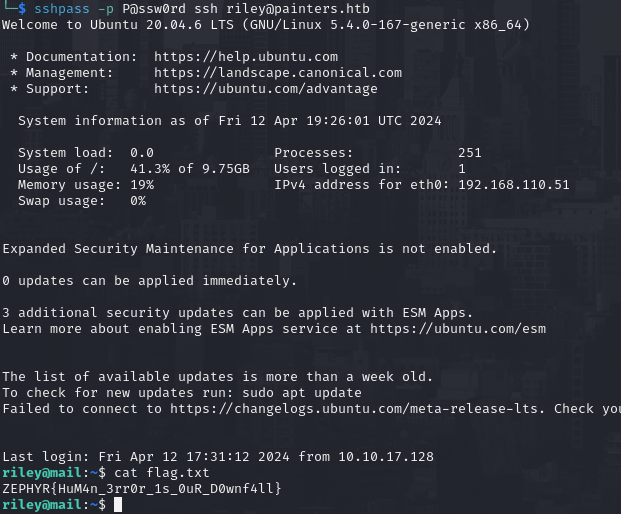
\includegraphics[width=\textwidth]{src/issues/5 - PREMONITION/issue54.png}
          \captionof{figure}{SSH and flag grabbing into the webserver}
          \label{5:PREMONITION:issue.md:issue54.png}
          \vspace{4ex}
        \end{minipage}
          
    \clearpage

    

\end{document}